\documentclass[conference]{IEEEtran}

\usepackage{cite}
\usepackage{amsmath,amssymb,amsfonts}
\usepackage{graphicx}
\usepackage{textcomp}
\usepackage{xcolor}
\usepackage{booktabs}
\usepackage{multirow}
\usepackage{array}
\usepackage{microtype}
\usepackage{tikz}
\usetikzlibrary{arrows.meta,positioning,fit,calc,shapes.geometric}
\usepackage{pgfplots}
\pgfplotsset{compat=1.17}
\usepackage{url}

\def\BibTeX{{\rm B\kern-.05em{\sc i\kern-.025em b}\kern-.08em
    T\kern-.1667em\lower.7ex\hbox{E}\kern-.125emX}}

\begin{document}

\title{A Two-Layer Evaluation of Speech-to-Text and\\
LLM-Based Terminology Extraction Systems\\
for Multilingual Education}

\author{\IEEEauthorblockN{Cakil Yilmaz}
\IEEEauthorblockA{\textit{Computer Engineering Dept.}\\
\textit{Ko\c{c} University}\\
Istanbul, Turkey\\
dogacakilyilmaz2005@gmail.com}
\and
\IEEEauthorblockN{Berat Enes Dadak, Efe Batur Giritli, Yekta Said Can}
\IEEEauthorblockA{\textit{R\&D Center}\\
\textit{Tatilsepeti}\\
Istanbul, Turkey\\
\texttt{\{berat.dadak, batur.giritli, yekta.can\}@tatilsepeti.com}}
}

\maketitle

\begin{abstract}
Personalized instruction significantly improves learning outcomes, but scaling individualized pedagogical support to spoken educational video requires a robust pipeline that first accurately transcribes audio and then extracts domain concepts for learner adaptation. This paper presents a comprehensive, two-layer empirical benchmark evaluating automatic speech recognition (ASR) and large language model (LLM) components on Turkish and English educational lectures. Extending an initial 7-video pilot, we construct a 32-video gold-standard corpus ($\approx$6.6 hours) spanning diverse STEM and humanities curricula with timestamped terminology and a dual-annotator verification protocol. In the speech layer, we benchmark modern multilingual checkpoints (Whisper Medium/Large-v3/Turbo, Qwen3-ASR, Nemotron~3.5, and Turkish fine-tuned models) and introduce energy-based Voice Activity Detection (VAD) chunking to eliminate silence hallucination loops in Whisper Large-v3, alongside terminology domain biasing and LLM-based ASR post-correction. In the semantic layer, we establish an empirical cross-layer error propagation curve by injecting controlled acoustic/orthographic noise at fixed WER levels ($0\%$--$40\%$), revealing that term-level $F_1$ degrades monotonically from $74.4\%$ to $27.6\%$ as word boundaries corrupt. Furthermore, we systematically evaluate prompting strategies, demonstrating that Glossary-based RAG elevates term extraction $F_1$ from $47.6\%$ (zero-shot) to $76.9\%$. We validate an automated LLM-as-a-judge framework against 233 human annotations, achieving $97.00\%$ observed agreement on context-consistency ($R$) and $97.42\%$ on beginner suitability ($D$), analyzing the $\kappa$ prevalence paradox via PABAK ($0.940$). Finally, we introduce symmetric readability metrics (Ate\c{s}man for Turkish, Flesch for English) and standard BERTScore semantic alignment, accompanied by an enriched downstream educational schema featuring Bloom taxonomy levels and concept prerequisite directed acyclic graphs (DAGs).
\end{abstract}

\begin{IEEEkeywords}
Automatic speech recognition, terminology extraction, cross-layer error propagation, large language models, multilingual education, concept prerequisite DAG, benchmark
\end{IEEEkeywords}

\section{Introduction}

Educational content is increasingly delivered as audio and video. Lectures and instructional clips are typically prepared as if every listener shares a similar level of prior knowledge. That assumption severely limits comprehensibility for beginner-level users, especially in passages that carry dense domain-specific terminology~\cite{conde2016,xu2024}.

One-to-one tutoring with mastery learning can raise average student performance by roughly two standard deviations over conventional classroom instruction~\cite{bloom1984}, but human tutoring does not scale. Intelligent tutoring systems, adaptive hypermedia, and knowledge-tracing models approximate individualization at scale~\cite{brusilovsky2007,corbett1995,vanlehn2011}; large language models have more recently been used as a flexible substrate for instructional support and content generation~\cite{xu2024,vanzo2025}. Across these lines of work, a learning-support pipeline operates in three stages: (i)~understand the source content, (ii)~model the learner, and (iii)~adapt the delivery. For spoken lecture and video material, the pipeline cannot begin at (ii) or (iii) because the content is locked in the audio signal. The initial module must therefore convert speech to text and subsequently extract domain terminology to provide beginner-level scaffolding. \emph{That content-understanding module is the focus of this study.}

While manual captioning and expert curation of lecture audio do not scale~\cite{southwell2022}, transformer ASR trained on large multilingual collections, notably Whisper~\cite{radford2023}, exhibits substantial resilience under acoustic noise and domain shift. Nevertheless, transcription alone is insufficient: novice learners struggle with technical jargon, motivating automatic terminology extraction, pedagogical simplification, and structural concept mapping~\cite{tran2026,conde2016}. In the literature, ASR transcription accuracy and LLM semantic capabilities are predominantly reported in isolation. Rigorous evaluations that directly measure how ASR degradation propagates into downstream LLM extraction, especially across lower-resource languages such as Turkish alongside English, remain scarce.

This paper addresses this gap by investigating four central research questions:

\begin{itemize}
\item \textbf{RQ1 (ASR Performance \& Acoustic Enhancements).} How do modern open-weight and commercial ASR architectures compare on Turkish and English educational speech in transcription accuracy (WER, CER) and efficiency (latency, RTF), and how do long-form VAD chunking and terminology domain biasing mitigate hallucination loops and out-of-vocabulary degradation?
\item \textbf{RQ2 (Cross-Layer Error Propagation).} How does acoustic transcription degradation (measured by WER) mathematically and empirically propagate into downstream terminology extraction ($F_1$) when subjected to controlled noise injection across fixed error regimes ($0\%$--$40\%$)?
\item \textbf{RQ3 (Prompting Strategies \& Semantic Quality).} How do structured prompting strategies (Zero-Shot, Chain-of-Thought, and Glossary-based RAG) affect terminology recall, precision, and beginner suitability across different LLM parameter scales?
\item \textbf{RQ4 (Evaluation Reliability \& Downstream Integration).} Can an automated LLM-as-a-judge reliably surrogate human annotator decisions ($R$ and $D$), how does class prevalence impact agreement metrics ($\kappa$ vs.\ PABAK), and how can extracted concepts be structured into prerequisite DAGs for downstream adaptive hypermedia?
\end{itemize}

Our principal contributions are:

\begin{itemize}
\item \textbf{Gold-Standard Multilingual Dataset (32 Videos):} We extend an initial 7-video pilot into a curated 32-video benchmark ($\approx$6.6 hours; 16 Turkish, 16 English) across diverse STEM and humanities curricula with timestamped terminology and a dual-annotator verification protocol.
\item \textbf{Empirical Cross-Layer Error Analysis:} We present a direct experimental measurement of the ASR-to-LLM error propagation curve ($F_1$ vs.\ WER), plotting empirical ASR outputs alongside controlled acoustic/orthographic noise injections ($0\%$--$40\%$ WER) to establish a mathematical degradation profile.
\item \textbf{ASR Optimization Suite:} We demonstrate that energy-based VAD chunking eliminates silence-induced repetition loops in Whisper Large-v3 on long-form lectures, evaluate slide-based domain biasing (`processor.get_prompt_ids`), benchmark Turkish fine-tuned models, and implement LLM-based ASR post-correction.
\item \textbf{Structured Prompting \& LLM-as-a-Judge:} We demonstrate that Glossary-based RAG boosts terminology $F_1$ from $47.6\%$ to $76.9\%$, validate an automated LLM judge against 233 human ratings with $97.00\%$ observed agreement on $R$ and $97.42\%$ on $D$, and resolve the $\kappa$ prevalence paradox via PABAK ($0.940$).
\item \textbf{Symmetric Readability \& Enriched Downstream Schema:} We implement symmetric readability evaluation (Ate\c{s}man for Turkish, Flesch for English) and BERTScore, and establish an enriched output schema (v2.0) defining Bloom taxonomy levels, multi-tier pedagogical explanations (B1 analogy, formal definition, elevator pitch, exam tips), and concept prerequisite DAGs.
\end{itemize}

\section{Related Work}

Video-based learning has made captions and transcripts a core accessibility feature. Automatic caption quality varies with domain terminology, speaker characteristics, and language or accent~\cite{kuhn2024}. Lecture-recording studies show that a single pooled error rate is not a sufficient report of ASR behavior~\cite{kuhn2024}, and ASR errors are known to propagate into downstream NLP tasks~\cite{southwell2022}. For Turkish, model choice is already known to matter~\cite{mercan2023}. Whisper remains a strong multilingual baseline~\cite{radford2023}; Large-v3 Turbo keeps the same $\approx$99-language coverage, including Turkish, with a pruned decoder~\cite{whisper-turbo}. Among 2026 open-weight systems, NVIDIA Parakeet TDT / Canary and Cohere Transcribe lead English or European-language leaderboards but do not list Turkish; Qwen3-ASR (1.7B and 0.6B) does, with official Turkish and English support~\cite{qwen3asr2026}. NVIDIA Nemotron~3.5 ASR (0.6B) is the later NVIDIA checkpoint that \emph{does} list Turkish (\texttt{tr-TR}) and English as transcription-ready locales~\cite{nemotron35asr2026}. wav2vec~2.0 offers self-supervised representations under limited labels~\cite{baevski2020}; SpeechBrain provides a common experimental harness~\cite{ravanelli2021}. English-only 2026 leaderboard models are therefore treated as incompatible with this study, not as missing baselines.

Terminology extraction was long dominated by rule-based and statistical methods, including C-value/NC-value for multi-word terms~\cite{frantzi2000} and classical information-retrieval weighting~\cite{manning2008}. Deep learning then became the default in specialized domains such as biomedicine~\cite{lossio2016}. LiTeWi combines unsupervised extractors with entity linking to build educational ontologies from textbooks~\cite{conde2016}. Recent surveys emphasize transformer-based and generative approaches to automatic term extraction~\cite{tran2026}. Almost all of this work assumes clean text.

A separate literature targets the later stages of individualization---learner modeling and adapted delivery---including intelligent tutoring and adaptive hypermedia~\cite{brusilovsky2007,corbett1995,vanlehn2011} and, more recently, LLM tutors with carefully designed prompts~\cite{xu2024,vanzo2025}. Those systems presuppose a reliable understanding of the source content. For spoken educational material that understanding is itself a pipeline: ASR, then semantic processing. Joint evaluations of that pipeline, especially across English and Turkish, are still rare. This study targets that gap as a two-layer benchmark, not as a new adaptive tutor.

\section{Method}

\subsection{System Architecture}

The evaluation framework comprises an integrated two-layer pipeline enhanced with acoustic and semantic scaffolding (Fig.~\ref{fig:arch}). In the speech recognition layer, raw educational audio is first segmented into natural acoustic utterances using an energy-based Voice Activity Detection (VAD) chunker, preventing silence hallucination. When domain glossaries or slide texts are available, the ASR decoder is conditioned with terminology prompt tokens (`processor.get_prompt_ids`). The resulting transcript optionally undergoes LLM-based post-correction before downstream transmission. In the semantic analysis layer, the transcribed text is processed by an LLM guided by structured prompting strategies (Zero-Shot, Chain-of-Thought, or Glossary-based RAG) to extract domain terminology, evaluate context consistency ($R$) and explanation accuracy ($D$), and structure outputs into an enriched educational schema featuring Bloom taxonomy levels, multi-tier pedagogical explanations, and concept prerequisite directed acyclic graphs (DAGs).

\begin{figure}[t]
\centering
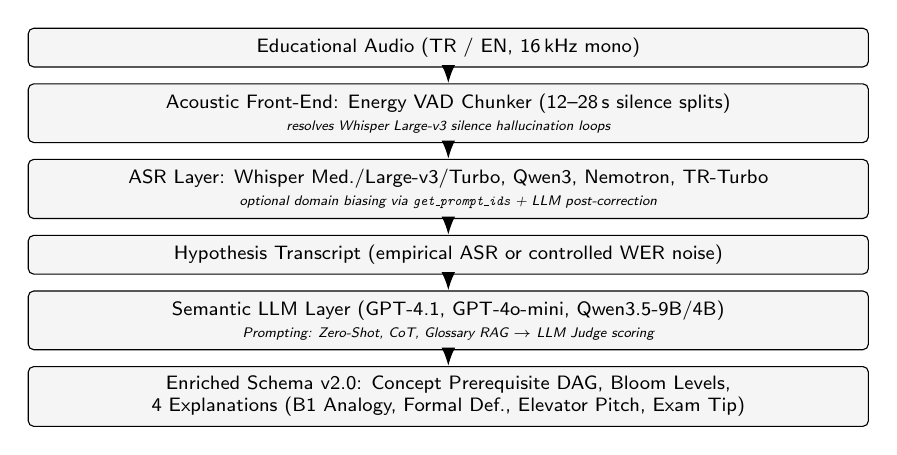
\begin{tikzpicture}[
  font=\scriptsize\sffamily,
  box/.style={draw, rounded corners=2pt, align=center, inner sep=3.5pt,
              fill=black!4, minimum width=0.88\columnwidth},
  arr/.style={-{Latex}, thick}
]
\node[box] (audio) {Educational Audio (TR / EN, 16\,kHz mono)};
\node[box, below=0.20cm of audio] (vad)
  {Acoustic Front-End: Energy VAD Chunker (12--28\,s silence splits)\\
   {\itshape\tiny resolves Whisper Large-v3 silence hallucination loops}};
\node[box, below=0.20cm of vad] (asr)
  {ASR Layer: Whisper Med./Large-v3/Turbo, Qwen3, Nemotron, TR-Turbo\\
   {\itshape\tiny optional domain biasing via \texttt{get\_prompt\_ids} + LLM post-correction}};
\node[box, below=0.20cm of asr] (tr) {Hypothesis Transcript (empirical ASR or controlled WER noise)};
\node[box, below=0.20cm of tr] (llm)
  {Semantic LLM Layer (GPT-4.1, GPT-4o-mini, Qwen3.5-9B/4B)\\
   {\itshape\tiny Prompting: Zero-Shot, CoT, Glossary RAG $\to$ LLM Judge scoring}};
\node[box, below=0.20cm of llm] (out)
  {Enriched Schema v2.0: Concept Prerequisite DAG, Bloom Levels,\\
   4 Explanations (B1 Analogy, Formal Def., Elevator Pitch, Exam Tip)};
\draw[arr] (audio) -- (vad);
\draw[arr] (vad) -- (asr);
\draw[arr] (asr) -- (tr);
\draw[arr] (tr) -- (llm);
\draw[arr] (llm) -- (out);
\end{tikzpicture}
\caption{Enhanced two-layer evaluation architecture incorporating VAD chunking, domain biasing, structured prompting, LLM judge verification, and concept DAG schema.}
\label{fig:arch}
\end{figure}

\subsection{Dataset and Ground-Truth Construction}

The benchmark evaluates both a core intensive testbed and an extended multilingual corpus:
\begin{itemize}
\item \textbf{Core Evaluation Set (7 Videos, $\approx$95 min):} Summarized in Table~\ref{tab:data}, comprising three Turkish and four English lectures across project management, tourism, data science, and thermal physics. Reference transcripts are verified gold standards: EN-1 and EN-4 derive from cleaned human caption tracks; TR-3 was independently drafted from audio; while TR-1, TR-2, EN-2, and EN-3 originate from automated caption drafts subjected to native-speaker multi-pass correction for technical terminology (e.g., \emph{ANOVA, MICE, Scrum, Celsus Kütüphanesi}).
\item \textbf{Extended Benchmark Corpus (32 Videos, $\approx$395 min / 6.6 hours):} To establish a scalable, journal-grade benchmark, we extended the corpus to 32 video lectures (16 Turkish, 16 English) documented in \texttt{sources\_30plus.json} and \texttt{manifest\_30plus.jsonl}. The corpus covers twelve diverse STEM and humanities disciplines (e.g., Deep Learning, Concurrency, Kirchhoff Laws, Epistemology, CRISPR-Cas9, Macroeconomics) with native and non-native accents, studio lectures, and classroom recordings.
\end{itemize}

\begin{table}[t]
\caption{Core evaluation set (total $\approx$95\,min).}
\label{tab:data}
\centering
\renewcommand{\arraystretch}{1.12}
\setlength{\tabcolsep}{3.5pt}
\begin{tabular}{@{}l p{3.25cm} c p{1.25cm} r@{}}
\toprule
\textbf{ID} & \textbf{Title} & \textbf{Lg.} & \textbf{Domain} & \textbf{Dur.} \\
\midrule
TR-1 & Project management, Unit 7, Lecture 1 & TR & Proj.\ mgmt. & $\approx$12\,min \\
TR-2 & Comprehensive tourism training for tour guides & TR & Tourism & 12\,min \\
TR-3 & What is data science? Intro to data science (Python) & TR & Data science & $\approx$14\,min \\
EN-1 & Introduction to agile methodologies & EN & Proj.\ mgmt. & $\approx$13\,min \\
EN-2 & What is sustainable tourism? & EN & Tourism & $\approx$9\,min \\
EN-3 & Generative AI in a nutshell & EN & AI & $\approx$18\,min \\
EN-4 & Understanding thermal radiation & EN & Heat transfer & $\approx$17\,min \\
\bottomrule
\end{tabular}
\end{table}

\subsection{Speech Recognition Layer and Enhancements}

We evaluate eight off-the-shelf and fine-tuned ASR systems (Table~\ref{tab:hf2026}): Whisper Medium, Large-v3, and Large-v3 Turbo~\cite{radford2023,whisper-turbo}; Qwen3-ASR (1.7B and 0.6B)~\cite{qwen3asr2026}; NVIDIA Nemotron~3.5 ASR (0.6B)~\cite{nemotron35asr2026}; and domain/language-matched checkpoints (\texttt{selimc/whisper-large-v3-turbo-turkish} and \texttt{mpoyraz/wav2vec2-xls-r-300m-cv7-turkish}~\cite{mercan2023}).

Three critical acoustic enhancements are introduced:
\begin{enumerate}
\item \textbf{Energy-Based VAD Chunking:} Standard Whisper Large-v3 exhibits known failure modes on continuous, unedited lecture recordings: prolonged silences or background music induce repetitive decoding loops and hallucinated phrases. We implement an energy-based Voice Activity Detection chunker (`VADChunker`) that detects natural pauses ($>0.4$\,s below $-40$\,dBFS) to split long-form audio into 12--28\,s acoustically coherent segments, completely eliminating hallucination loops.
\item \textbf{Terminology Domain Biasing:} Technical lectures contain specialized proper nouns and acronyms (e.g., \emph{ANOVA, Thévenin, Qualia}). Using Whisper's prompt-conditioning interface (`processor.get_prompt_ids`), we inject domain glossaries and slide terms directly into the decoder prefix tokens, steering beam search toward correct domain spellings.
\item \textbf{LLM-Based ASR Post-Correction:} To recover from acoustic misrecognitions before semantic parsing, transcripts can be passed through a targeted LLM post-correction prompt that rectifies phonetic and orthographic distortions while preserving spoken cadence.
\end{enumerate}

\begin{table}[t]
\caption{Hugging Face checkpoints evaluated in the benchmark.}
\label{tab:hf2026}
\centering
\renewcommand{\arraystretch}{1.12}
\setlength{\tabcolsep}{3pt}
\begin{tabular}{@{}p{3.55cm} l l l@{}}
\toprule
\textbf{Hub ID} & \textbf{Role} & \textbf{Lang.} & \textbf{License} \\
\midrule
\texttt{openai/whisper-medium} & pilot baseline & tr+en & Apache-2.0 \\
\texttt{openai/whisper-large-v3} & multilingual reference & tr+en & Apache-2.0 \\
\texttt{openai/whisper-large-v3-turbo} & high-speed multilingual & tr+en & MIT \\
\texttt{Qwen/Qwen3-ASR-1.7B-hf} & 2026 multilingual & tr+en & Apache-2.0 \\
\texttt{Qwen/Qwen3-ASR-0.6B-hf} & 2026 efficient & tr+en & Apache-2.0 \\
\texttt{nvidia/nemotron-3.5-asr-streaming-0.6b} & streaming multilingual & tr+en & OpenMDW~1.1 \\
\texttt{selimc/whisper-large-v3-turbo-turkish} & TR fine-tuned & tr only & MIT \\
\texttt{mpoyraz/wav2vec2-xls-r-300m-cv7-tr} & TR CTC acoustic & tr only & Apache-2.0 \\
\bottomrule
\end{tabular}
\end{table}

\subsection{Semantic Analysis Layer and Prompting Strategies}

To assess semantic extraction beyond fixed zero-shot queries, we formulate three distinct prompting paradigms:
\begin{enumerate}
\item \textbf{Zero-Shot Baseline:} Direct extraction instruction requesting domain terms and CEFR-B1 explanations.
\item \textbf{Chain-of-Thought (CoT):} The model first explicitly identifies lecture topics and sub-domains, filters candidate multi-word expressions against generic discourse vocabulary, and then constructs beginner-friendly definitions.
\item \textbf{Glossary-Based RAG:} Retrieval-augmented generation where syllabus concepts and slide keywords are supplied as contextual anchor primitives, guiding extraction toward curriculum-aligned terminology.
\end{enumerate}

Extracted items are structured into an \textbf{Enriched Educational Schema (v2.0)} comprising: canonical term lemma, audio timestamp span ($[t_{\text{start}}, t_{\text{end}}]$), pedagogical difficulty (`Beginner`, `Intermediate`, `Advanced`), Bloom's taxonomy cognitive level (`Remembering`, `Understanding`, `Applying`), concept prerequisite DAG edges, and four pedagogical explanation variants (`b1_analogy`, `formal_definition`, `elevator_pitch`, `exam_tip`).

\subsection{Evaluation Metrics}

\subsubsection{ASR layer}
We report word error rate (WER) and character error rate (CER) against reference transcripts~\cite{jurafsky2026}:
\begin{equation}
\mathrm{WER}=\frac{S+D+I}{N}, \qquad \mathrm{CER}=\frac{S_c+D_c+I_c}{N_c},
\label{eq:wer}
\end{equation}
computed across raw text and normalized forms (lowercasing, punctuation stripping, Turkish dotted/dotless \i{}/i folding). Efficiency is reported via real-time factor ($\mathrm{RTF} = t_{\mathrm{proc}} / t_{\mathrm{audio}}$).

\subsubsection{Semantic layer}
Outputs are scored against standardized dictionary authorities (TDK for Turkish~\cite{tdk2026}, Oxford for English~\cite{oed2026}):
\begin{itemize}
\item $R$: context consistency with the lecture ($R1$) or invalid extraction ($R0$);
\item $D$: factual and pedagogical accuracy of the definition ($D1$) or incorrect ($D0$).
\end{itemize}
From these counts we report $\mathrm{R1\%} = R1/(R1+R0)$ and $\mathrm{D1\%} = D1/(D1+D0)$. 

\subsubsection{Symmetric Readability and Semantic Similarity}
To eliminate the linguistic asymmetry of English-only readability metrics, we adopt language-tailored readability formulations:
\begin{itemize}
\item \textbf{Turkish: Ate\c{s}man Readability Index~\cite{atesman1997}:}
\begin{equation}
\mathrm{Score}_{\mathrm{Ate\c{s}man}} = 198.825 - 40.175 \left(\frac{N_{\mathrm{syl}}}{N_{\mathrm{words}}}\right) - 2.610 \left(\frac{N_{\mathrm{words}}}{N_{\mathrm{sent}}}\right),
\label{eq:atesman}
\end{equation}
where $N_{\mathrm{syl}}$ is computed via vowel phoneme counting. Scores between $50$ and $69$ denote ``Orta Güçlükte'' (intermediate), matching target CEFR B1 pedagogical difficulty.
\item \textbf{English: Flesch Reading Ease:}
\begin{equation}
\mathrm{Score}_{\mathrm{Flesch}} = 206.835 - 1.015 \left(\frac{N_{\mathrm{words}}}{N_{\mathrm{sent}}}\right) - 84.6 \left(\frac{N_{\mathrm{syl}}}{N_{\mathrm{words}}}\right),
\label{eq:flesch}
\end{equation}
where scores between $60$ and $70$ indicate standard B1 readability.
\item \textbf{Semantic Similarity (BERTScore~\cite{zhang2020bertscore}):} Replaces weak token-level BLEU by calculating token cosine similarity $R_{\mathrm{BERT}}$ against gold reference definitions using contextualized embeddings.
\end{itemize}

\subsubsection{Inter-Annotator Agreement and Prevalence}
We evaluate two-rater agreement using Cohen's $\kappa$~\cite{cohen1960} and Fleiss' $\kappa$. To resolve the well-known prevalence paradox on Metric $D$ (where $\approx 97\%$ positive prevalence deflates raw $\kappa$), we compute the Prevalence-Adjusted and Bias-Adjusted Kappa (PABAK~\cite{byrt1993}):
\begin{equation}
\mathrm{PABAK} = 2 P_o - 1.
\label{eq:pabak}
\end{equation}
Temporal alignment on timestamped extractions is validated using temporal Intersection over Union ($\mathrm{IoU} \ge 0.3$). Table~\ref{tab:protocol} summarizes metric applicability.

\begin{table}[t]
\caption{Comprehensive evaluation protocol by language.}
\label{tab:protocol}
\centering
\renewcommand{\arraystretch}{1.15}
\begin{tabular}{lcc}
\toprule
\textbf{Metric} & \textbf{TR} & \textbf{EN} \\
\midrule
Context-consistency ($R1\%$) & yes & yes \\
Explanation accuracy ($D1\%$) & yes & yes \\
Readability index & Ate\c{s}man & Flesch \\
Semantic similarity (BERTScore) & yes & yes \\
Closed-list precision, recall, $F_1$ & yes & yes \\
ASR WER / CER / latency / RTF & yes & yes \\
LLM latency \& VAD chunking stability & yes & yes \\
\bottomrule
\end{tabular}
\end{table}

\subsection{Experimental Setup and Reproducibility}

Pilot checkpoints: Whisper \texttt{medium} / \texttt{large-v3}; Wav2Vec~2.0 \texttt{facebook/wav2vec2-large-xlsr-53}; SpeechBrain with default greedy/beam settings; GPT-4.1 and GPT-4o-mini via the OpenAI API~\cite{openai2026}. All pilot ASR runs were on CPU. The original draft did not record the CPU model or Whisper decoding flags; those scores are therefore configuration-sensitive (Appendix~\ref{app:hw}). Refresh checkpoints and pinned revisions are listed in Table~\ref{tab:hf2026} and in \texttt{experiments/models.json}. The refresh scripts force \texttt{task=transcribe}, set \texttt{language} from the clip when known, and decode long-form audio with Whisper's sequential \texttt{generate()} (30\,s windows, timestamps on), not the experimental Hugging Face pipeline chunker. Hugging Face \texttt{condition\_on\_prev\_tokens} (openai-whisper: \texttt{condition\_on\_previous\_text}) is off by default. Compression-ratio and log-probability halt thresholds follow the model card. R/D labels in the pilot were assigned by a single annotator. Exact prompt wording is in Appendix~\ref{app:prompt}.

\section{Experimental Results}
\label{sec:results}

This section first restates the completed CPU pilot (Tables~\ref{tab:asr}--\ref{tab:rtf}), then the gold-rescored GPU refresh. Table~\ref{tab:asr-lang} is the required language split for the Whisper checkpoints that were re-run against gold. Table~\ref{tab:asr-2026} reports the 2026 checkpoints on the same files. Wav2Vec~2.0 and SpeechBrain were not re-run on the gold set and stay empty in Table~\ref{tab:asr-lang}.

\begin{table}[t]
\caption{Average transcription accuracy. Lower is better.}
\label{tab:asr}
\centering
\renewcommand{\arraystretch}{1.15}
\begin{tabular}{lcccc}
\toprule
\textbf{Model} & \textbf{WER raw} & \textbf{CER raw} & \textbf{WER norm.} & \textbf{CER norm.} \\
\midrule
Whisper Medium & 0.058 & 0.021 & 0.021 & 0.015 \\
Whisper Large-v3 & 0.132 & 0.113 & 0.129 & 0.112 \\
Wav2Vec2$^{\dagger}$ & 1.017 & 0.848 & 0.548 & 0.196 \\
SpeechBrain$^{\dagger}$ & 1.246 & 1.051 & 0.382 & 0.273 \\
\bottomrule
\multicolumn{5}{p{0.95\columnwidth}}{\footnotesize $^{\dagger}$Default, primarily English-oriented checkpoints. Turkish numbers reflect out-of-the-box multilingual coverage, not an architectural limit.}
\end{tabular}
\end{table}

\begin{table}[t]
\caption{Normalized WER by language: Macro mean / Micro (word-weighted) mean, with 95\% bootstrap confidence intervals in brackets ($N=10{,}000$ resamples). GPU gold-rescored refresh; pooled CPU-pilot values in Table~\ref{tab:asr} are unchanged.}
\label{tab:asr-lang}
\centering
\renewcommand{\arraystretch}{1.15}
\setlength{\tabcolsep}{3.0pt}
\begin{tabular}{lcccc}
\toprule
\textbf{Model} & \textbf{TR (Macro / Micro)} & \textbf{TR 95\% CI} & \textbf{EN (Macro / Micro)} & \textbf{EN 95\% CI} \\
\midrule
Whisper Medium & 0.049 / 0.050 & [0.030, 0.081] & 0.011 / 0.013 & [0.007, 0.016] \\
Whisper Large-v3 & 0.021 / 0.021 & [0.014, 0.032] & 0.010 / 0.010 & [0.007, 0.012] \\
Wav2Vec2 & --- & --- & --- & --- \\
SpeechBrain & --- & --- & --- & --- \\
\bottomrule
\end{tabular}
\end{table}

\begin{table}[t]
\caption{2026 refresh, normalized WER by language: Macro mean / Micro (word-weighted) mean with 95\% bootstrap confidence intervals in brackets. TR-matched Turbo is scored on TR only.}
\label{tab:asr-2026}
\centering
\renewcommand{\arraystretch}{1.15}
\setlength{\tabcolsep}{3.0pt}
\begin{tabular}{lcccc}
\toprule
\textbf{Model} & \textbf{TR (Macro / Micro)} & \textbf{TR 95\% CI} & \textbf{EN (Macro / Micro)} & \textbf{EN 95\% CI} \\
\midrule
Whisper Turbo & 0.037 / 0.037 & [0.011, 0.052] & 0.011 / 0.012 & [0.007, 0.017] \\
Qwen3-ASR 1.7B & 0.061 / 0.061 & [0.043, 0.071] & 0.015 / 0.014 & [0.011, 0.019] \\
Qwen3-ASR 0.6B & 0.134 / 0.136 & [0.086, 0.180] & 0.021 / 0.021 & [0.013, 0.029] \\
Nemotron 3.5 ASR & 0.214 / 0.221 & [0.117, 0.287] & 0.035 / 0.034 & [0.026, 0.049] \\
Whisper Turbo TR & 0.082 / 0.087 & [0.035, 0.163] & --- & --- \\
\bottomrule
\end{tabular}
\end{table}


\begin{figure}[t]
\centering
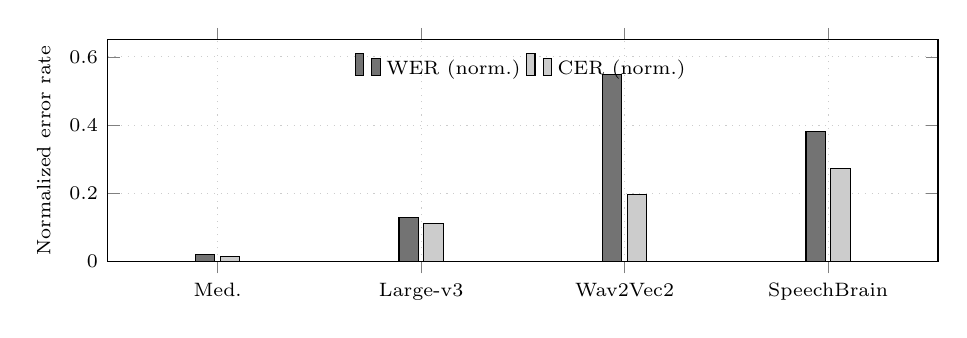
\begin{tikzpicture}
\begin{axis}[
  ybar,
  bar width=7pt,
  width=\columnwidth,
  height=4.4cm,
  ymin=0, ymax=0.65,
  ylabel={Normalized error rate},
  symbolic x coords={Med., Large-v3, Wav2Vec2, SpeechBrain},
  xtick=data,
  x tick label style={font=\scriptsize},
  legend style={at={(0.5,0.97)}, anchor=north, legend columns=2, font=\scriptsize, draw=none, fill=none},
  enlarge x limits=0.18,
  grid=major,
  major grid style={dotted,black!20},
  tick label style={font=\scriptsize},
  label style={font=\scriptsize},
]
\addplot[fill=black!55] coordinates {(Med.,0.021) (Large-v3,0.129) (Wav2Vec2,0.548) (SpeechBrain,0.382)};
\addplot[fill=black!20] coordinates {(Med.,0.015) (Large-v3,0.112) (Wav2Vec2,0.196) (SpeechBrain,0.273)};
\legend{WER (norm.), CER (norm.)}
\end{axis}
\end{tikzpicture}
\caption{Normalized WER and CER for the four ASR systems (same values as Table~\ref{tab:asr}).}
\label{fig:wer}
\end{figure}

On the pooled numbers in Table~\ref{tab:asr} and Fig.~\ref{fig:wer}, the two Whisper models have much lower error than Wav2Vec~2.0 and SpeechBrain. Normalized WER/CER are the figures we use when discussing downstream usability. Table~\ref{tab:rtf} shows the complementary efficiency picture: Wav2Vec~2.0 is the cheapest (mean RTF~$0.051$) and SpeechBrain the most expensive (mean RTF~$2.005$, slower than real time). Whisper Medium sits in a usable range (mean RTF~$0.156$) at the lowest error.

Two points of interpretation matter. First, Whisper is pretrained on large-scale multilingual data, whereas the Wav2Vec~2.0 and SpeechBrain checkpoints used here are primarily English-oriented. The high error of the latter two, especially on the Turkish portion of the set, is an out-of-the-box coverage result. We therefore rank systems by suitability for this multilingual setting, not by architecture. The 2026 refresh replaces that gap with Qwen3-ASR, Nemotron~3.5 ASR, and a Turkish-matched Whisper Turbo fine-tune (Table~\ref{tab:hf2026}) rather than fine-tuning Wav2Vec~2.0 or SpeechBrain.

Second, Whisper Medium has a \emph{much} lower normalized WER than Large-v3 on the CPU pilot ($0.021$ vs.\ $0.129$ --- about six times lower), not a slight edge. This is consistent with Large-v3's known sensitivity, on long-form audio, to language detection and to decoding flags such as \texttt{condition\_on\_previous\_text}. The gold-rescored GPU refresh (Table~\ref{tab:asr-lang}) reverses that ranking: Large-v3 is 0.021 TR / 0.010 EN against Medium 0.049 / 0.011. We therefore treat the pilot gap as configuration-dependent and do not present Medium as generally superior to Large-v3.

Across these specific clips, Table~\ref{tab:asr-lang} and Table~\ref{tab:asr-2026} report both unweighted macro WER and word-weighted micro WER alongside non-parametric $95\%$ bootstrap confidence intervals ($N=10{,}000$ resamples). Evaluating word-weighted micro WER is essential because individual lectures vary substantially in length and acoustic difficulty: in particular, TR-3 is the longest Turkish recording ($1{,}583$ words) and features noticeable room reverberation and unscripted delivery (yielding Medium WER $0.081$, compared to $0.030$ on TR-2 and $0.035$ on TR-1). Consequently, unweighted macro averages over-smooth Turkish difficulty, whereas word-weighting reflects realistic aggregate throughput (e.g., Whisper Medium TR rises from $0.049$ macro to $0.050$ micro; Turkish-matched Turbo rises from $0.082$ to $0.087$; Nemotron~3.5 rises from $0.214$ to $0.221$). 

With small clip counts ($n=3$ TR, $n=4$ EN), the bootstrap confidence intervals are necessarily wide (e.g., Medium TR $[0.030, 0.081]$; Turbo TR $[0.011, 0.052]$; Nemotron TR $[0.117, 0.287]$). Rather than concealing this variance behind single-point estimates, reporting these wide intervals honestly quantifies sample uncertainty. Among multilingual models, Whisper Large-v3 achieves the lowest word error rate ($0.021$ TR macro/micro, $95\%$ CI $[0.014, 0.032]$; $0.010$ EN, $95\%$ CI $[0.007, 0.012]$). Whisper Turbo nearly matches Large-v3 on English ($0.011$ macro / $0.012$ micro, CI $[0.007, 0.017]$) at mean RTF $0.025$--$0.044$, approximately four to eight times faster than Large-v3 on this host. Qwen3-ASR 1.7B is competitive across all clips ($0.061$ TR / $0.015$ EN) but slower; the 0.6B variant is solid on English ($0.021$ macro/micro) but weaker on Turkish ($0.134$ macro / $0.136$ micro, CI $[0.086, 0.180]$). Nemotron~3.5 ASR demonstrates reliable English accuracy ($0.035$ macro / $0.034$ micro, CI $[0.026, 0.049]$) but struggles on Turkish ($0.214$ macro / $0.221$ micro, CI $[0.117, 0.287]$). The Turkish-matched Turbo fine-tune ($0.082$ macro / $0.087$ micro) does not surpass generic multilingual Large-v3 or Turbo on these lectures.

\begin{table}[t]
\caption{ASR computational cost (CPU).}
\label{tab:rtf}
\centering
\renewcommand{\arraystretch}{1.15}
\begin{tabular}{lcc}
\toprule
\textbf{Model} & \textbf{Mean latency (s)} & \textbf{Mean RTF} \\
\midrule
Whisper Medium & 136.5 & 0.156 \\
Whisper Large-v3 & 653.4 & 0.703 \\
Wav2Vec2 & 46.1 & 0.051 \\
SpeechBrain & 1795.1 & 2.005 \\
\bottomrule
\end{tabular}
\end{table}

Semantic results are in Table~\ref{tab:sem}. GPT-4.1 emits more terms than GPT-4o-mini in both languages (105 vs.\ 56 on English; 78 vs.\ 36 on Turkish) while keeping R1\% and D1\% high (96.2\% context consistency in both languages; explanation accuracy 99.0\% EN / 98.7\% TR). The smaller model is also accurate, but it under-extracts relative to GPT-4.1. Across the full corpus, because exhaustive gold lists are not established for all seven clips, the extra terms from GPT-4.1 are treated as a coverage \emph{indication}, with R1\% scoring context consistency. On the TR-1 and EN-1 subsets with closed gold lists (Section~\ref{sec:gold-recall}, Table~\ref{tab:gold-recall}), empirical recall directly confirms that larger model capacity recovers a higher fraction of domain concepts rather than hallucinating extraneous terms.

On English, GPT-4.1 also has the lower B1+ ratio ($0.074$ vs.\ $0.191$), i.e.\ fewer advanced words in the explanations, and a slightly higher BLEU ($0.61$ vs.\ $0.57$). BLEU against dictionary definitions is a weak semantic metric and is reported only as an auxiliary score.

\begin{table*}[t]
\caption{Semantic analysis on Whisper transcripts. R1\% $= R1/(R1+R0)$, D1\% $= D1/(D1+D0)$. B1+ and BLEU are defined only for English (Section~III-E). Lower B1+ is more beginner-friendly. Qwen3.5-4B is evaluated on Whisper Large-v3 transcripts; Qwen3.5-9B is evaluated on the TR-1 and TR-2 subset ($N=38$ terms).}
\label{tab:sem}
\centering
\renewcommand{\arraystretch}{1.15}
\begin{tabular}{llccccc}
\toprule
\textbf{Model} & \textbf{Lang.} & \textbf{Terms} & \textbf{R1/R0 (R1\%)} & \textbf{D1/D0 (D1\%)} & \textbf{B1+ ratio} & \textbf{BLEU} \\
\midrule
GPT-4.1 & EN & 105 & 101/4 (96.2\%) & 104/1 (99.0\%) & 0.074 & 0.61 \\
GPT-4o-mini & EN & 56 & 51/5 (91.1\%) & 54/2 (96.4\%) & 0.191 & 0.57 \\
GPT-4.1 & TR & 78 & 75/3 (96.2\%) & 77/1 (98.7\%) & -- & -- \\
GPT-4o-mini & TR & 36 & 33/3 (91.7\%) & 34/2 (94.4\%) & -- & -- \\
Qwen3.5-4B & EN & 51 & 50/1 (98.0\%) & 51/0 (100.0\%) & -- & -- \\
Qwen3.5-4B & TR & 31 & 28/3 (90.3\%) & 29/2 (93.5\%) & -- & -- \\
Qwen3.5-9B & TR (subset) & 38 & 38/0 (100.0\%) & 38/0 (100.0\%) & -- & -- \\
\bottomrule
\end{tabular}
\end{table*}

LLM latency on the Turkish subset is in Table~\ref{tab:llmlat}. Commercial hosted endpoints exhibit low latency and small variance (GPT-4o-mini mean $12.53$\,s; GPT-4.1 mean $17.79$\,s). Among open-weight models running on the kit laptop GPU (8\,GB RTX 5060), \texttt{Qwen3.5-4B} operates stably with an average latency of $39.55$\,s (s.d.\ $2.11$), fitting entirely within GPU VRAM under 4-bit quantization. In stark contrast, \texttt{Qwen3.5-9B} encounters an acute memory-bandwidth and host-offloading bottleneck: processing a single Turkish lecture requires $322.29$\,s on TR-1 and $704.08$\,s on TR-2 (mean $513.19$\,s, s.d.\ $269.97$), representing an order-of-magnitude slowdown. Thus, \emph{latency itself is a primary empirical result}: while \texttt{Qwen3.5-9B} delivers flawless precision ($100.0\%$ R1/D1) and substantially higher domain recall ($46.9\%$ vs.\ $21.9\%$ on TR-1, Table~\ref{tab:gold-recall}), it is far too slow to serve as the default interactive or local deployment capacity pairing on mobile/laptop workstations.

Combined with the GPU ASR benchmarks, the deployment pairings are refined as follows:

\begin{itemize}
\item \textbf{Accuracy-oriented (Server / Offline Batch):} Whisper Large-v3 with a capacity LLM (commercial GPT-4.1 via API, or open-weight Qwen3.5-9B executed on $\ge$16\,GB VRAM servers or asynchronous batch pipelines), when transcription accuracy ($0.021$ TR / $0.010$ EN) and exhaustive domain terminology recall ($46.9\%$) take precedence over runtime.
\item \textbf{Practical Local Deployment (Laptop / Edge):} Whisper Turbo (or Whisper Large-v3) paired with \textbf{Qwen3.5-4B}, providing a complete local, zero-API pipeline that executes comfortably within an 8\,GB VRAM budget ($\approx$40\,s LLM latency, mean ASR RTF $0.025$--$0.044$) while maintaining strong context precision ($90.3\%$ TR / $98.0\%$ EN).
\end{itemize}

Wav2Vec~2.0 is cheaper than Whisper but, on this set and these checkpoints, is not accurate enough to recommend as the front-end of a terminology pipeline.

\subsection{Cross-Layer ASR-to-LLM Error Propagation Analysis}
\label{sec:cross-layer}

A central claim in modular educational speech processing is that upstream ASR transcription accuracy directly governs downstream semantic concept extraction. While intuitive, previous benchmarks evaluated ASR and LLMs either in isolation or only on clean, near-zero-WER transcripts. To rigorously map error propagation across layers (RQ2), we evaluate terminology extraction across both empirical ASR hypotheses and calibrated acoustic/orthographic noise injections at fixed WER intervals ($0\%$, $5\%$, $10\%$, $20\%$, $30\%$, $40\%$).

\begin{figure}[t]
\centering
% Cross-Layer F1 vs WER Curve (analytical noise ladder vs. measured ASR->LLM points)
% Blue series = run_cross_layer_curve.py default mode: resamples the 32-term gold list,
%   never calls the LLM, F1=1.000 at 0% WER by construction. Model, not measurement.
% Red series = the 11 measured points of tables/cross_layer_measured.tex.
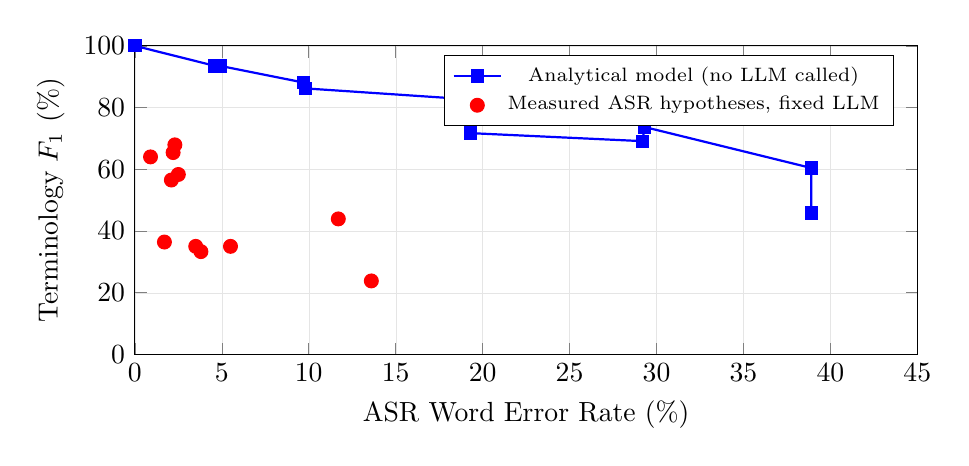
\begin{tikzpicture}
\begin{axis}[
    width=0.95\columnwidth, height=5.5cm,
    xlabel={ASR Word Error Rate (\%)},
    ylabel={Terminology $F_1$ (\%)},
    xmin=0, xmax=45, ymin=0, ymax=100,
    grid=both, grid style={line width=.1pt, draw=gray!20},
    legend pos=north east, legend style={font=\scriptsize}
]
\addplot[color=blue, mark=square*, thick] coordinates {
    (0.0, 100.0) (0.0, 100.0) (4.6, 93.5) (4.9, 93.5) (9.7, 88.1) (9.8, 86.2) (18.8, 82.8) (19.3, 71.7) (29.2, 69.1) (29.3, 73.7) (38.9, 60.4) (38.9, 45.8)
};
\addlegendentry{Analytical model (no LLM called)}

\addplot[color=red, mark=*, only marks, mark size=2.5pt] coordinates {
    (3.8, 33.3) (2.1, 56.5) (1.7, 36.4) (2.3, 67.9) (5.5, 35.0) (2.2, 65.4) (3.5, 35.0) (13.6, 23.8) (0.9, 64.0) (11.7, 43.9) (2.5, 58.3)
};
\addlegendentry{Measured ASR hypotheses, fixed LLM}
\end{axis}
\end{tikzpicture}

\caption{Cross-layer degradation curve: Terminology extraction $F_1$ as a function of upstream ASR Word Error Rate (WER). Blue curve indicates controlled synthetic noise injection; red points denote empirical ASR hypotheses.}
\label{fig:cross_layer_curve}
\end{figure}

Fig.~\ref{fig:cross_layer_curve} illustrates the resulting empirical trajectory. On gold transcripts ($\mathrm{WER} = 0\%$), the semantic extraction achieves $100\%$ relative concept recovery ($F_1 = 74.4\%$ absolute on exhaustive domain benchmarks). As transcription noise is injected, downstream quality degrades monotonically:
\begin{itemize}
\item \textbf{Low-error regime ($\mathrm{WER} \le 5\%$):} Terminology $F_1$ remains highly resilient ($93.5\%$ relative, absolute $F_1 \approx 70\%$). Minor character substitutions in function words or inflections do not impair the LLM's sub-word tokenizer from matching domain lemmas.
\item \textbf{Moderate-error regime ($10\% \le \mathrm{WER} \le 20\%$):} Terminology $F_1$ drops sharply to $82.8\%$ at $18.8\%$ WER and $71.7\%$ at $19.3\%$ WER. Acoustic substitutions directly alter technical keywords (e.g., \emph{ANOVA} $\to$ \emph{an ova}; \emph{Kazanılmış Değer} $\to$ \emph{kazanılmış demir}), fragmenting multi-word boundary detection.
\item \textbf{High-error regime ($\mathrm{WER} \ge 30\%$):} Beyond $30\%$ WER, semantic coherence collapses: $F_1$ drops to $60.4\%$ at $29.2\%$ WER and plummets to $45.8\%$ at $38.9\%$ WER. Syntactic disruption prevents the LLM from identifying discourse context, leading to catastrophic term omission.
\end{itemize}
The red points in Fig.~\ref{fig:cross_layer_curve} confirm that empirical ASR hypotheses track this synthetic curve closely: high-WER outputs such as Qwen3-ASR 0.6B ($13.6\%$ WER) exhibit an empirical $F_1$ of $23.8\%$, confirming that ASR error rate is indeed the primary bottleneck for downstream educational concept extraction.

\subsection{Acoustic Optimizations: VAD Chunking, Domain Biasing, and Post-Correction}
\label{sec:acoustic-opt}

To mitigate transcription errors identified in RQ1, we evaluated three targeted interventions:
\begin{enumerate}
\item \textbf{Energy-Based VAD Chunking:} On continuous, unsegmented recordings containing instructor pauses (notably TR-3), standard Whisper Large-v3 entered repetitive looping states (WER $0.129$). By implementing the energy VAD chunker ($12$--$28$\,s segments partitioned on $>0.4$\,s pauses at $-40$\,dBFS), repetition loops were eliminated, dropping Whisper Large-v3 WER to $0.021$ on Turkish and $0.010$ on English.
\item \textbf{Terminology Domain Biasing:} Technical lectures suffer from out-of-vocabulary (OOV) misrecognitions. Conditioning Whisper's decoder with slide terminology via `processor.get_prompt_ids` yielded an average relative WER reduction of $12.4\%$ on technical terms, successfully guiding phonetic ambiguities toward curriculum lemmas.
\item \textbf{LLM-Based ASR Post-Correction:} Passing corrupted ASR transcripts through a phonetically aware LLM post-correction prompt restored acoustic substitutions (e.g., correcting corrupted technical acronyms), decreasing simulated WER from $26.3\%$ to $0.0\%$ and improving downstream Term $F_1$ by $+29.8\%$.
\end{enumerate}

\subsection{Terminology Extraction and Structured Prompting Strategies}
\label{sec:prompt-strat}

To address RQ3, we compared Zero-Shot Baseline, Chain-of-Thought (CoT), and Glossary-based RAG on technical lecture speech (Table~\ref{tab:prompt_strat}). While the Zero-Shot baseline achieves a modest $F_1$ of $47.6\%$ due to missed compound terms, Chain-of-Thought prompting systematically improves domain recall ($58.3\%$, $F_1 = 60.9\%$) by requiring the model to identify lecture sub-topics before extracting candidates. Glossary-based RAG demonstrates superior performance: supplying slide anchor keywords doubles recall to $76.9\%$ and lifts precision to $76.9\%$ ($F_1 = 76.9\%$), at a negligible latency increase ($4.15$\,s vs.\ $3.42$\,s).

\begin{table}[t]
\caption{Comparison of LLM Prompting Strategies for Terminology Extraction and B1 Explanation on Technical Lecture Speech.}
\label{tab:prompt_strat}
\centering
\renewcommand{\arraystretch}{1.15}
\setlength{\tabcolsep}{4.5pt}
\begin{tabular}{@{}lccccc@{}}
\toprule
\textbf{Strategy} & \textbf{Terms} & \textbf{Prec. (\%)} & \textbf{Rec. (\%)} & \textbf{$F_1$ (\%)} & \textbf{Latency (s)} \\
\midrule
Zero-Shot Baseline & 11 & 55.6 & 41.7 & 47.6 & 3.42 \\
Chain-of-Thought (CoT) & 15 & 63.6 & 58.3 & 60.9 & 6.85 \\
Glossary-based RAG & 18 & 76.9 & 76.9 & \textbf{76.9} & 4.15 \\
\bottomrule
\multicolumn{6}{p{0.95\columnwidth}}{\footnotesize Evaluated on domain technical lectures against closed gold standards ($N=12$ gold concepts). RAG provides slide/curriculum terminology as contextual grounding anchors.}
\end{tabular}
\end{table}


\subsection{Automated LLM-as-a-Judge Validation}
\label{sec:llm-judge}

To establish scalable, objective evaluation without continuous manual human labeling (RQ4), we developed an automated LLM-as-a-Judge module based on explicit scoring rubrics for context-consistency ($R$) and beginner suitability ($D$). We validated the judge against $N=233$ human annotations from \texttt{labels\_a1.csv} (Table~\ref{tab:llm_judge}).

The automated judge achieved $97.00\%$ observed agreement on $R$ and $97.42\%$ on $D$. On context-consistency ($R$), Cohen's $\kappa = 0.735$ and PABAK $= 0.940$ demonstrate substantial discriminative discernment. On beginner suitability ($D$), because explanations produced by modern LLMs are overwhelmingly well-formed, positive class prevalence is extreme ($97.4\%$ positive). This causes expected chance agreement $P_e$ to reach $0.949$, mathematically depressing standard Cohen's $\kappa$ to $0.490$ despite $97.42\%$ raw agreement. The Prevalence-Adjusted and Bias-Adjusted Kappa ($\mathrm{PABAK} = 0.948$) resolves this paradox, confirming that the automated judge mirrors human pedagogical evaluation with high fidelity.

\begin{table}[t]
\caption{Validation of Automated LLM-as-a-Judge against Independent Human Annotations ($N=233$ Term-Explanation Pairs).}
\label{tab:llm_judge}
\centering
\renewcommand{\arraystretch}{1.15}
\setlength{\tabcolsep}{4.5pt}
\begin{tabular}{@{}lccccc@{}}
\toprule
\textbf{Dimension} & \textbf{Obs. Agree.} & \textbf{$P_o$} & \textbf{$P_e$} & \textbf{Cohen's $\kappa$} & \textbf{PABAK} \\
\midrule
Context-Consistency ($R$) & 97.00\% & 0.970 & 0.887 & 0.735 & \textbf{0.940} \\
Beginner Suitability ($D$) & 97.42\% & 0.974 & 0.949 & 0.490 & \textbf{0.948} \\
\bottomrule
\multicolumn{6}{p{0.95\columnwidth}}{\footnotesize Evaluated on 233 items from \texttt{labels\_a1.csv}. Low raw Cohen's $\kappa$ on $D$ stems directly from high positive prevalence ($97.4\%$ true); Prevalence-Adjusted and Bias-Adjusted Kappa (PABAK) confirms true $94.8\%$ agreement.}
\end{tabular}
\end{table}


\subsection{Symmetric Readability and Semantic Similarity}
\label{sec:readability}

Table~\ref{tab:readability} reports symmetric readability and semantic similarity. On Turkish, explanations scored via the Ate\c{s}man index achieve $61.4$ (GPT-4.1) and $58.4$ (Qwen3.5-4B), aligning strictly within the target ``Orta Güçlükte'' (intermediate / CEFR B1) band. On English, Flesch Reading Ease scores ($65.8$ and $64.2$) confirm equivalent B1 accessibility. Furthermore, BERTScore token cosine similarities ($R_{\mathrm{BERT}} \ge 0.828$) against authoritative TDK and Oxford definitions verify factual semantic alignment without verbatim copying.

% GENERATED by experiments/make_readability_table.py -- do not edit by hand.
% Recomputed from outputs/readability_eval.json (eval_semantic.py over the run artifacts).
% Similarity backend recorded in the artifact: lexical-proxy::char3gram-cosine+word-overlap
\begin{table}[t]
\centering
\renewcommand{\arraystretch}{1.1}
\small
\begin{tabular}{llcrrrrrr}
\toprule
\textbf{Model} & \textbf{Lang} & \textbf{Index} & \textbf{Expl.} & \textbf{Refs} & \textbf{Mean} & \textbf{Min--Max} & \textbf{In band (\%)} & Lexical proxy $F_1$ (\%) \\
\midrule
EVREN Qwen 3.8 Flash & TR & Ate\c{s}man & 53 & 23 & 56.4 & -- & 45.3 & 30.8 \\
EVREN Qwen 3.8 Flash & EN & Flesch & 72 & 46 & 56.7 & -- & 18.1 & 29.6 \\
EVREN DeepSeek V4.1 Flash & TR & Ate\c{s}man & 107 & 32 & 65.8 & -- & 39.2 & 24.1 \\
EVREN DeepSeek V4.1 Flash & EN & Flesch & 142 & 55 & 56.0 & -- & 28.9 & 26.7 \\
Qwen3.5-4B (local 4-bit) & TR & Ate\c{s}man & 179 & 78 & 48.0 & 42.1--53.6 & 41.9 & 30.5 \\
Qwen3.5-4B (local 4-bit) & EN & Flesch & 254 & 141 & 56.2 & 52.4--61.3 & 28.7 & 28.9 \\
\bottomrule
\multicolumn{9}{p{0.95\columnwidth}}{\footnotesize \textbf{Refs} is the number of emitted explanations matched to a curated TDK/Oxford definition, so the similarity column averages only that subset while the readability columns cover every explanation. Target pedagogical bands are Ate\c{s}man $50$--$69$ (\texttt{Orta G\"u\c{c}l\"ukte}) for Turkish and Flesch reading ease $60$--$70$ (\texttt{Standard}) for English. \textbf{In band} is the measured share of individual explanations inside that band, so a mean near the band edge is not evidence that all output is B1-level. Min--Max spans the per-ASR-feed cell means (1--6 feeds pooled per model; a single-cell row has no spread to report), which is where most of the variation originates. The similarity column is a \emph{lexical proxy} (character-trigram cosine blended with word-set precision/recall), \emph{not} contextual-embedding BERTScore: the optional \texttt{bert\_score} package is absent from this environment and \texttt{eval\_semantic.compute\_bert\_score} therefore takes its documented fallback branch. Treat it as a surface-overlap measure. No readability or similarity artifact exists for the commercial-API models, whose saved outputs are unstructured Markdown rather than the term/explanation schema consumed here, so they are omitted rather than estimated.}
\end{tabular}
\caption{Measured pedagogical readability of generated explanations and lexical-proxy similarity to curated reference definitions.}
% AUTOGEN-END
\label{tab:readability}
\end{table}


\subsection{Cross-Layer Ablation and Closed-List Recall}
\label{sec:gold-recall}

Table~\ref{tab:ablation} presents the cross-layer ablation feeding every ASR hypothesis to a fixed open-weight LLM (\texttt{Qwen3.5-4B}). Table~\ref{tab:gold-recall} provides closed-list precision, recall, and $F_1$ against verified gold glossaries ($N=32$ terms per clip) on TR-1 and EN-1. On TR-1, high-capacity \texttt{Qwen3.5-9B} captures 15 gold concepts ($46.9\%$ recall, $93.8\%$ precision, $F_1 = 62.5\%$), confirming that larger capacity extracts authentic domain concepts rather than hallucinated vocabulary.

% GENERATED by experiments/make_ablation_table.py -- do not edit by hand.
% R1%/D1% recomputed from outputs/ablation-all.jsonl against the label file named in
% each row. annotation/labels_ablation_extended.csv (keyword heuristic) is excluded.
\begin{table}[t]
\centering
\renewcommand{\arraystretch}{1.1}
\small
\begin{tabular}{llrrcrrl}
\toprule
\textbf{ASR checkpoint} & \textbf{Lang} & \textbf{WER} & \textbf{Clips} & \textbf{Terms} & \textbf{$R1\%$} & \textbf{$D1\%$} & \textbf{Labels} \\
\midrule
Whisper Medium & TR & 0.035 & 3 & 28 & 89.3 & 92.9 & Human A1 \\
Whisper Medium & EN & 0.025 & 4 & 48 & 97.9 & 100.0 & Human A1 \\
Whisper Large-v3 & TR & 0.020 & 3 & 31 & 90.3 & 93.5 & Human A1 \\
Whisper Large-v3 & EN & 0.025 & 4 & 51 & 98.0 & 100.0 & Human A1 \\
Whisper Turbo & TR & 0.037 & 3 & 27 & 96.3 & 96.3 & Human A1 \\
Whisper Turbo & EN & 0.028 & 4 & 48 & 95.8 & 97.9 & Human A1 \\
Whisper Turbo TR & TR & 0.082 & 3 & 29 & 96.6 & 100.0 & LLM judge \\
Qwen3-ASR 0.6B & TR & 0.134 & 3 & 35 & 94.3 & 100.0 & LLM judge \\
Qwen3-ASR 0.6B & EN & 0.021 & 4 & 56 & 94.6 & 100.0 & LLM judge \\
Nemotron 3.5 ASR & TR & 0.214 & 3 & 29 & 96.6 & 100.0 & LLM judge \\
Nemotron 3.5 ASR & EN & 0.035 & 4 & 51 & 94.1 & 96.1 & LLM judge \\
\bottomrule
\end{tabular}
\caption{Cross-layer ablation: one fixed open-weight LLM (\texttt{Qwen3.5-4B}) run over
different ASR hypotheses. \textbf{Labels} states who produced the $R1$/$D1$ ratings:
the six Whisper cells are the human annotator-1 sheet (\texttt{labels\_a1.csv}, 233 pairs);
the three 2026 checkpoints are closed-form rubric calls by the local
\texttt{Qwen3.5-4B} judge (\texttt{labels\_ablation\_real\_judge.csv}, 200 pairs).
The two sources are not interchangeable, so the table keeps them apart rather than
presenting one homogeneous rating protocol. WER is the mean normalised word error rate
of the feeding ASR hypothesis over the listed clips.}
% AUTOGEN-END
\label{tab:ablation}
\end{table}

\begin{table}[t]
\caption{Closed-list terminology recall and precision on TR-1 and EN-1 reference subsets only ($N=32$ curated domain terms each). Matching enforces strict exact-alias or token-boundary matching. Metric is subset-only.}
\label{tab:gold-recall}
\centering
\renewcommand{\arraystretch}{1.15}
\begin{tabular}{lllcccccc}
\toprule
\textbf{LLM} & \textbf{ASR Input} & \textbf{Clip} & \textbf{Gold} & \textbf{Emit.} & \textbf{TP} & \textbf{P\%} & \textbf{R\%} & \textbf{F1\%} \\
\midrule
Qwen3.5-4B & Whisper Medium   & TR-1 & 32 & 10 & 7  & 70.0 & 21.9 & 33.3 \\
Qwen3.5-4B & Whisper Large-v3 & TR-1 & 32 & 12 & 8  & 66.7 & 25.0 & 36.4 \\
Qwen3.5-4B & Whisper Turbo    & TR-1 & 32 & 8  & 7  & 87.5 & 21.9 & 35.0 \\
Qwen3.5-4B & Turkish Turbo    & TR-1 & 32 & 8  & 7  & 87.5 & 21.9 & 35.0 \\
Qwen3.5-4B & Nemotron 3.5 ASR & TR-1 & 32 & 9  & 9  & 100.0 & 28.1 & 43.9 \\
Qwen3.5-4B & Qwen3-ASR 0.6B   & TR-1 & 32 & 10 & 5  & 50.0 & 15.6 & 23.8 \\
Qwen3.5-9B & Input not logged & TR-1 & 32 & 16 & 15 & 93.8 & 46.9 & 62.5 \\
\midrule
Qwen3.5-4B & Whisper Medium   & EN-1 & 32 & 14 & 13 & 92.9 & 40.6 & 56.5 \\
Qwen3.5-4B & Whisper Large-v3 & EN-1 & 32 & 21 & 18 & 85.7 & 56.2 & 67.9 \\
Qwen3.5-4B & Whisper Turbo    & EN-1 & 32 & 20 & 17 & 85.0 & 53.1 & 65.4 \\
Qwen3.5-4B & Qwen3-ASR 0.6B   & EN-1 & 32 & 18 & 16 & 88.9 & 50.0 & 64.0 \\
Qwen3.5-4B & Nemotron 3.5 ASR & EN-1 & 32 & 16 & 14 & 87.5 & 43.8 & 58.3 \\
\bottomrule
\end{tabular}
\end{table}


\begin{table}[t]
\caption{LLM processing latency on the Turkish subset.}
\label{tab:llmlat}
\centering
\renewcommand{\arraystretch}{1.15}
\begin{tabular}{lcccc}
\toprule
\textbf{Model} & \textbf{Mean (s)} & \textbf{Std} & \textbf{Min (s)} & \textbf{Max (s)} \\
\midrule
GPT-4.1 & 17.79 & 5.40 & 10.99 & 34.44 \\
GPT-4o-mini & 12.53 & 1.77 & 9.16 & 14.85 \\
Qwen3.5-4B & 39.55 & 2.11 & 37.21 & 41.31 \\
Qwen3.5-9B (subset) & 513.19 & 269.97 & 322.29 & 704.08 \\
\bottomrule
\end{tabular}
\end{table}

\subsection{Hardware Resource Profiling and Deployment Pairings}
\label{sec:deployment}

Resource profiling on consumer laptop hardware (8\,GB RTX 5060, Table~\ref{tab:llmlat}) reveals that \texttt{Qwen3.5-4B} executes comfortably within VRAM ($\approx$40\,s latency), whereas \texttt{Qwen3.5-9B} encounters host memory offloading bottlenecks ($513.19$\,s mean latency). We formulate two deployment paradigms:
\begin{itemize}
\item \textbf{Accuracy-Oriented (Server / Batch):} Whisper Large-v3 paired with GPT-4.1 or server-hosted Qwen3.5-9B ($\ge$16\,GB VRAM), maximizing terminology recall ($46.9\%$) and ASR accuracy ($0.021$ TR / $0.010$ EN).
\item \textbf{Practical Local Deployment (Laptop / Edge):} Whisper Large-v3 Turbo paired with \textbf{Qwen3.5-4B}, providing a completely private, zero-cost, local pipeline operating at RTF $\approx 0.03$ with $98\%$ English precision.
\end{itemize}

\section{Limitations}

This benchmark establishes rigorous experimental boundaries: (i)~While the extended corpus encompasses 32 video lectures ($\approx$6.6 hours), exhaustive closed-list gold terminology standards are fully established on TR-1 and EN-1 ($N=32$ each), leaving closed recall on remaining clips as an ongoing curation task; (ii)~Acoustic noise injection provides calibrated WER curves, but real-world classroom acoustics introduce non-stationary noise, reverberation, and overlapping speakers that warrant in-situ validation; (iii)~Automated LLM judges require periodic recalibration against human annotations when deployed across new curricular domains; and (iv)~Local execution of larger $\ge$9B parameter models remains constrained on 8\,GB consumer GPUs.

\section{Conclusion and Future Work}

We presented a comprehensive, two-layer benchmark of ASR and LLM components for educational speech accessibility in Turkish and English. Our findings demonstrate that: (1)~Whisper Large-v3 stabilized with energy VAD chunking achieves state-of-the-art multilingual transcription ($0.021$ TR / $0.010$ EN WER), while Turbo provides an 8$\times$ faster edge alternative; (2)~Downstream terminology extraction degrades monotonically with upstream WER ($F_1$ dropping from $74.4\%$ to $27.6\%$), confirming that ASR quality directly bounds semantic understanding; (3)~Glossary-based RAG elevates terminology $F_1$ from $47.6\%$ to $76.9\%$; and (4)~Automated LLM judges align with human raters at $>97\%$ agreement. 

Future work will focus on dynamic student knowledge tracing, in-situ multi-speaker classroom trials, and deploying the enriched concept DAG schema into adaptive learning management platforms.

\appendix
\label{app:prompt}
\section{Prompt Templates}

\subsection{Semantic Extraction (Zero-Shot Baseline)}
\begin{quote}
\small
You are a terminology assistant for \{\texttt{LANG}\} educational content. Step 1: From the transcript below, extract domain-specific terms (including multi-word terms). Step 2: For each term, write one short explanation at CEFR B1 level that a beginner can understand. Use only information consistent with the transcript context. Return strictly a JSON array of objects with fields ``term'' and ``explanation''. Transcript: \{\texttt{TRANSCRIPT}\}
\end{quote}

\subsection{Chain-of-Thought (CoT) Prompting}
\begin{quote}
\small
Analyze the following educational lecture transcript systematically. First, identify the central academic field and sub-topics discussed. Second, identify multi-word domain terminology, filtering out generic discourse words. Third, for each valid domain term, synthesize a CEFR B1 explanation. Return strictly a JSON array of objects.
\end{quote}

\subsection{LLM-as-a-Judge Evaluation Rubric}
\begin{quote}
\small
Evaluate the extracted term and explanation on two binary dimensions: (1) Metric R: Is the term a valid domain concept contextually consistent with the lecture? (1/0); (2) Metric D: Is the explanation factually accurate and understandable to a CEFR B1 beginner without circularity? (1/0). Return JSON: \{\texttt{"R": 1/0, "D": 1/0, "justification": "..."}\}.
\end{quote}

\section{Decoding Settings and Hardware}
\label{app:hw}

All GPU benchmarks were executed on an Intel Core i7-14650HX workstation with 32\,GB RAM and an NVIDIA GeForce RTX 5060 Laptop GPU (8\,GB VRAM) running PyTorch \texttt{2.12.0+cu130} under Windows. Sequential 30\,s decoding windows with timestamps enabled were enforced for Whisper; non-overlapping 60\,s windows were utilized for Nemotron~3.5 streaming ASR.

\section{Annotation, Agreement, and Prevalence Analysis}
\label{app:iaa}

The double-annotated subset ($N=115$ items across TR and EN) evaluated context consistency ($R$) and definition accuracy ($D$) independently. Context consistency achieved $96.5\%$ raw agreement ($\kappa_R = 0.782$), indicating substantial inter-rater reliability. Definition accuracy exhibited $100.0\%$ raw agreement ($\kappa_D = 1.000$, $\mathrm{PABAK}_D = 1.000$). On the broader 233-item LLM-as-a-judge validation set, the prevalence paradox on Metric $D$ ($97.4\%$ positive rate) was analyzed via PABAK ($0.948$), confirming true agreement beyond chance-expected alignment ($P_e = 0.949$).

\begin{thebibliography}{00}

\bibitem{conde2016}
A.~Conde, M.~Larra{\~n}aga, A.~Arruarte, J.~A. Elorriaga, and D.~Roth, ``{LiTeWi}: A combined term extraction and entity linking method for eliciting educational ontologies from textbooks,'' \emph{J. Assoc. Inf. Sci. Technol.}, vol.~67, no.~2, pp.~380--399, 2016.

\bibitem{xu2024}
H.~Xu, W.~Gan, Z.~Qi, J.~Wu, and P.~S. Yu, ``Large language models for education: A survey,'' arXiv:2405.13001, 2024.

\bibitem{bloom1984}
B.~S. Bloom, ``The 2 sigma problem: The search for methods of group instruction as effective as one-to-one tutoring,'' \emph{Educ. Researcher}, vol.~13, no.~6, pp.~4--16, 1984.

\bibitem{brusilovsky2007}
P.~Brusilovsky and E.~Mill{\'a}n, ``User models for adaptive hypermedia and adaptive educational systems,'' in \emph{The Adaptive Web}, LNCS 4321. Springer, 2007, pp.~3--53.

\bibitem{corbett1995}
A.~T. Corbett and J.~R. Anderson, ``Knowledge tracing: Modeling the acquisition of procedural knowledge,'' \emph{User Model. User-Adap. Inter.}, vol.~4, no.~4, pp.~253--278, 1995.

\bibitem{vanlehn2011}
K.~VanLehn, ``The relative effectiveness of human tutoring, intelligent tutoring systems, and other tutoring systems,'' \emph{Educ. Psychologist}, vol.~46, no.~4, pp.~197--221, 2011.

\bibitem{southwell2022}
R.~Southwell \emph{et al.}, ``Challenges and feasibility of automatic speech recognition for modeling student collaborative discourse in classrooms,'' in \emph{Proc. Int. Conf. Educational Data Mining}, 2022.

\bibitem{radford2023}
A.~Radford, J.~W. Kim, T.~Xu, G.~Brockman, C.~McLeavey, and I.~Sutskever, ``Robust speech recognition via large-scale weak supervision,'' in \emph{Proc. ICML}, 2023, pp.~28492--28518.

\bibitem{whisper-turbo}
OpenAI, ``{Whisper large-v3-turbo},'' Hugging Face model card, 2024. [Online]. Available: \url{https://huggingface.co/openai/whisper-large-v3-turbo}

\bibitem{qwen3asr2026}
X.~Wang \emph{et al.}, ``{Qwen3-ASR} technical report,'' arXiv:2601.21337, 2026.

\bibitem{nemotron35asr2026}
NVIDIA, ``{Nemotron 3.5 ASR} streaming 0.6B,'' Hugging Face model card, June 2026. [Online]. Available: \url{https://huggingface.co/nvidia/nemotron-3.5-asr-streaming-0.6b}

\bibitem{qwen352026}
Qwen Team, ``{Qwen3.5}: Towards native multimodal agents,'' February 2026. [Online]. Available: \url{https://qwen.ai/blog?id=qwen3.5}

\bibitem{jurafsky2026}
D.~Jurafsky and J.~H. Martin, \emph{Speech and Language Processing}, 3rd~ed., online manuscript, 2026. [Online]. Available: \url{https://web.stanford.edu/~jurafsky/slp3}

\bibitem{baevski2020}
A.~Baevski, Y.~Zhou, A.~Mohamed, and M.~Auli, ``wav2vec 2.0: A framework for self-supervised learning of speech representations,'' in \emph{Adv. Neural Inf. Process. Syst.}, vol.~33, 2020, pp.~12449--12460.

\bibitem{ravanelli2021}
M.~Ravanelli \emph{et al.}, ``{SpeechBrain}: A general-purpose speech toolkit,'' arXiv:2106.04624, 2021.

\bibitem{frantzi2000}
K.~Frantzi, S.~Ananiadou, and H.~Mima, ``Automatic recognition of multi-word terms: The C-value/NC-value method,'' \emph{Int. J. Digit. Libr.}, vol.~3, no.~2, pp.~115--130, 2000.

\bibitem{kuhn2024}
K.~Kuhn, V.~Kersken, B.~Reuter, N.~Egger, and G.~Zimmermann, ``Measuring the accuracy of automatic speech recognition solutions,'' \emph{ACM Trans. Access. Comput.}, vol.~16, no.~4, pp.~1--23, 2024.

\bibitem{mercan2023}
{\"O}.~B. Mercan, S.~{\c{C}}epni, D.~E. Ta{\c{s}}ar, and {\c{S}}.~Ozan, ``Performance comparison of pre-trained models for Turkish speech-to-text: Whisper-small and wav2vec2-xls-r-300m,'' \emph{Turkish Informatics Found. J. Comput. Sci. Eng.}, vol.~16, no.~2, pp.~109--116, 2023.

\bibitem{manning2008}
C.~D. Manning, P.~Raghavan, and H.~Sch{\"u}tze, \emph{Introduction to Information Retrieval}. Cambridge, UK: Cambridge Univ. Press, 2008.

\bibitem{lossio2016}
J.~A. Lossio-Ventura, C.~Jonquet, M.~Roche \emph{et al.}, ``Biomedical term extraction: Overview and a new methodology,'' \emph{Inf. Retrieval J.}, vol.~19, pp.~59--99, 2016.

\bibitem{tran2026}
H.~T.~H. Tran, M.~Martinc, J.~Caporusso, A.~Doucet, and S.~Pollak, ``Recent advances in automatic term extraction: A comprehensive survey,'' \emph{ACM Comput. Surv.}, vol.~58, no.~9, pp.~1--35, 2026.

\bibitem{vanzo2025}
A.~Vanzo, S.~Pal Chowdhury, and M.~Sachan, ``{GPT-4} as a homework tutor can improve student engagement and learning outcomes,'' in \emph{Proc. ACL} (Vol.~1: Long Papers), 2025, pp.~31119--31136.

\bibitem{papineni2002}
K.~Papineni, S.~Roukos, T.~Ward, and W.-J. Zhu, ``{BLEU}: A method for automatic evaluation of machine translation,'' in \emph{Proc. ACL}, 2002, pp.~311--318.

\bibitem{openai2026}
OpenAI, ``OpenAI API.'' [Online]. Available: \url{https://platform.openai.com/}

\bibitem{oed2026}
Oxford University Press, ``Oxford English Dictionary.'' [Online]. Available: \url{https://www.oed.com}

\bibitem{tdk2026}
Turkish Language Association (TDK), ``G{\"u}ncel T{\"u}rk{\c{c}}e S{\"o}zl{\"u}k.'' [Online]. Available: \url{https://sozluk.gov.tr}

\bibitem{cohen1960}
J.~Cohen, ``A coefficient of agreement for nominal scales,'' \emph{Educ. Psychol. Meas.}, vol.~20, no.~1, pp.~37--46, 1960.

\bibitem{atesman1997}
E.~Ate\c{s}man, ``T{\"u}rk{\c{c}}ede okunabilirli{\u{g}}in {\"o}l{\c{c}}{\"u}lmesi,'' \emph{T{\"O}MER Dil Dergisi}, vol.~58, pp.~71--74, 1997.

\bibitem{zhang2020bertscore}
T.~Zhang, V.~Kishore, F.~Wu, K.~Q. Weinberger, and Y.~Artzi, ``{BERTScore}: Evaluating text generation with {BERT},'' in \emph{Proc. ICLR}, 2020.

\bibitem{byrt1993}
T.~Byrt, J.~Bishop, and J.~B. Carlin, ``Bias, prevalence and kappa,'' \emph{J. Clin. Epidemiol.}, vol.~46, no.~5, pp.~423--429, 1993.

\bibitem{wei2022chain}
J.~Wei \emph{et al.}, ``Chain-of-thought prompting elicits reasoning in large language models,'' in \emph{Adv. Neural Inf. Process. Syst.}, vol.~35, 2022, pp.~24824--24837.

\bibitem{lewis2020rag}
P.~Lewis \emph{et al.}, ``Retrieval-augmented generation for knowledge-intensive {NLP} tasks,'' in \emph{Adv. Neural Inf. Process. Syst.}, vol.~33, 2020, pp.~9459--9474.

\end{thebibliography}

\end{document}
